%%===========================================================%%
%%                                                           %%
%%                       MONTE CARLO                         %%
%%                                                           %%
%%===========================================================%%


\chapter{Monte Carlo simulations}\label{chap:mc}

This chapter contains description of MC generators and MC samples used for determination of signal event reconstruction and selection efficiency (Sec.~\ref{sec:mcExclusiveSignal}), modelling of background contribution (Sec.~\ref{sec:mcBkgdContrib}), and comparison of hadron level cross sections with model predictions (Sec.~\ref{sec:mcModelPred}). Apart from described samples also single particles ($\pi$, $K$, $p$) embedded into zero-bias data were used for the purpose of the TPC and TOF reconstruction efficiency calculations, but their description is ommited here as related calculations were presented in Ref.~\cite{supplementaryNote}.

\section{Exclusive signal}\label{sec:mcExclusiveSignal}

\subsection{GenEx $\pi^{+}\pi^{-}$ embedded into zero-bias data}

Signal sample with exclusive $\pi^{+}\pi^{-}$ was prepared with GenEx\cite{GenEx} event generator. Each event has been passed independently through Geant3 simulation of the STAR detector (STARsim) and Geant4 simulation of the RP Phase II* detectors, merged at the end and fully embedded into the same zero-bias data event. Before passing through the STAR detector model, events were filtered in order to gain production efficiency. At the particle level pions were required to have $p_{T}>0.15$~GeV and $|\eta|<1$, while forward scattered protons (after added beam divergence) were required to fit within fiducial region envelope (Eq.~\eqref{eq:RpFiducial}) extended by 3 standard deviations of the angular beam divergence.

%moze napisac ile przypadkow

\subsection{Forward scattered protons embedded into zero-bias data}

Specially for determination of the RP track reconstruction and selection efficiency independent, large sample of forward scattered protons from GenEx was simulated in Geant4 and embedded into zero-bias data.


\subsection{Fast MC generator for particle identification studies}
Correction reflecting efficiency of identification requires good modeling of detector response in terms of $dE/dx$ and TOF time ($\rightarrow m^{2}_{\text{TOF}}$) measurement which were used for this purpose as described in Sec.~\ref{subsec:pidCuts}. In addition to this, significant number of simulated events is needed to reduce statistical uncertainties of efficiency. The former was provided by adjusting $dE/dx$ spectra from embedded MC to match the data, as elaborated in Chap.~7 of Ref.~\cite{supplementaryNote}. The latter, however, was not easy to achieve for exclusive $K^{+}K^{-}$ and $p\bar{p}$ whose identification is most challenging and information about identification efficiency is the most needed among studied species. Specially for study of particle (exlusive pair) identification a dedicated MC simulation was prepared.

This dedicated MC simulation was designed to work as follows (simulation of single CEP event of predefined pair ID is described):
\begin{enumerate}
 \item The position of $z_{\text{vtx}}$ was drawn from predefined distribution.
 \item Kinematics of central state particles was set: momentum (magnitude) $p$, pseudorapidity $\eta$ and azimuthal angle $\phi$ of positive and negative charge particles were drawn from predefined distributions.
 \item Both particles were tested if doubled radius of curvature $2R$ of associated track in the magnetic field of the TPC ($B=0.5$~T, $R \propto p_{\text{T}}/B$) is smaller than the radius of TOF detector barell (assumed 212~cm). If not then event was skipped and procedure was restared (back to 1.).
 \item The particles were propagated from the vertex at $(0,0,z_{\text{vtx}})$ through the magnetic field of TPC using Newton's method with the time step (in the laboratory) equal 100~ps, corresponding to space step $<3$~cm.
 \item After step 4. the position of the TOF cell was known allowing to calculate the TOF path length $L$ between the vertex and position of the TOF hit. Also the TOF hit time $t$ was then known, further smeared by adding random number from normal distribution with mean at 0 and standard deviation $\sigma_{\text{TOF}}=60$~ps to account for the finite TOF time measurement resolution. In addition to this, reconstructed tracks' (transverse) momenta were defined as the true momenta smeared by 6~MeV if $p_{\text{T}}<0.3$~GeV or by $2.4~\text{MeV} + 1.2\%\times p_{\text{T}}$ if $p_{\text{T}}>0.3$~GeV, to account for finite TPC momentum resolution. At this stage it was possible to calculate $m^{2}_{\text{TOF}}$ using Eq.~\eqref{eq:mSquared}.
 \item The $dE/dx$ measurement was simulated. For each particle a $dE/dx$ was drawn from the distribution of the form given by Eq.~(7.6) and of parameters (for given particle ID and momentum) which were extracted from the data and tabulated in Tab.~7.1, all contained in Chap.~7 of Ref.~\cite{supplementaryNote}. This assured that the simulated $dE/dx$ exactly matched the data. Once $dE/dx$ for both particles (tracks) was obtained, value of the $dE/dx$ error (more strictly: uncertainty of $\ln(dE/dx~[\text{keV/cm}])$) and value of $\log_{2}(dx)$ was also set up. These quantities depend on the number of TPC hit points used in the reconstruction of $dE/dx$ (the more hits in tracks, the better resolution of $dE/dx$ and higher $dx$), which obviously is not accessible without full STAR simulation in Geant. This problem was solved by extracting dependence of $\sigma(\ln(dE/dx))$ and $\log_{2}(dx)$ on the TOF path length from the data (from CEP events, Fig.~\ref{fig:correlationsTofPathLength}). Since the length of the TOF path is very strongly correlated with the number of hits forming the track and thus number of hits used to reconstruct $dE/dx$, one is allowed to draw $\sigma(\ln(dE/dx))$ and $\log_{2}(dx)$ from their distributions for particular TOF path lengths calculated in 5. and use as measured ones. In this way the simulation preserves relevant connections between $dE/dx$-related quantities. After these steps are taken the $n\sigma_{X}$ ($X=\pi$, $K$, $p$) variables are calculated for each track using the definition (Eq.~\eqref{eq:nSigmaDef}), in exactly the same way as it is done during standard data reconstruction.
 \item Event information needed to study pair identification was stored in the ROOT tree: ID of particles forming a pair, their three-momenta, $m^{2}_{\text{TOF}}$, $n\sigma_{\pi}$, $n\sigma_{K}$ and $n\sigma_{p}$.
\end{enumerate}

%--------------------------- 
\begin{figure}%[ht!] 
\centering
\parbox{0.4725\textwidth}{
  \centering
  \begin{subfigure}[b]{\linewidth}{
                \subcaptionbox{\label{fig:dEdxErrorVsTofPathLength}}{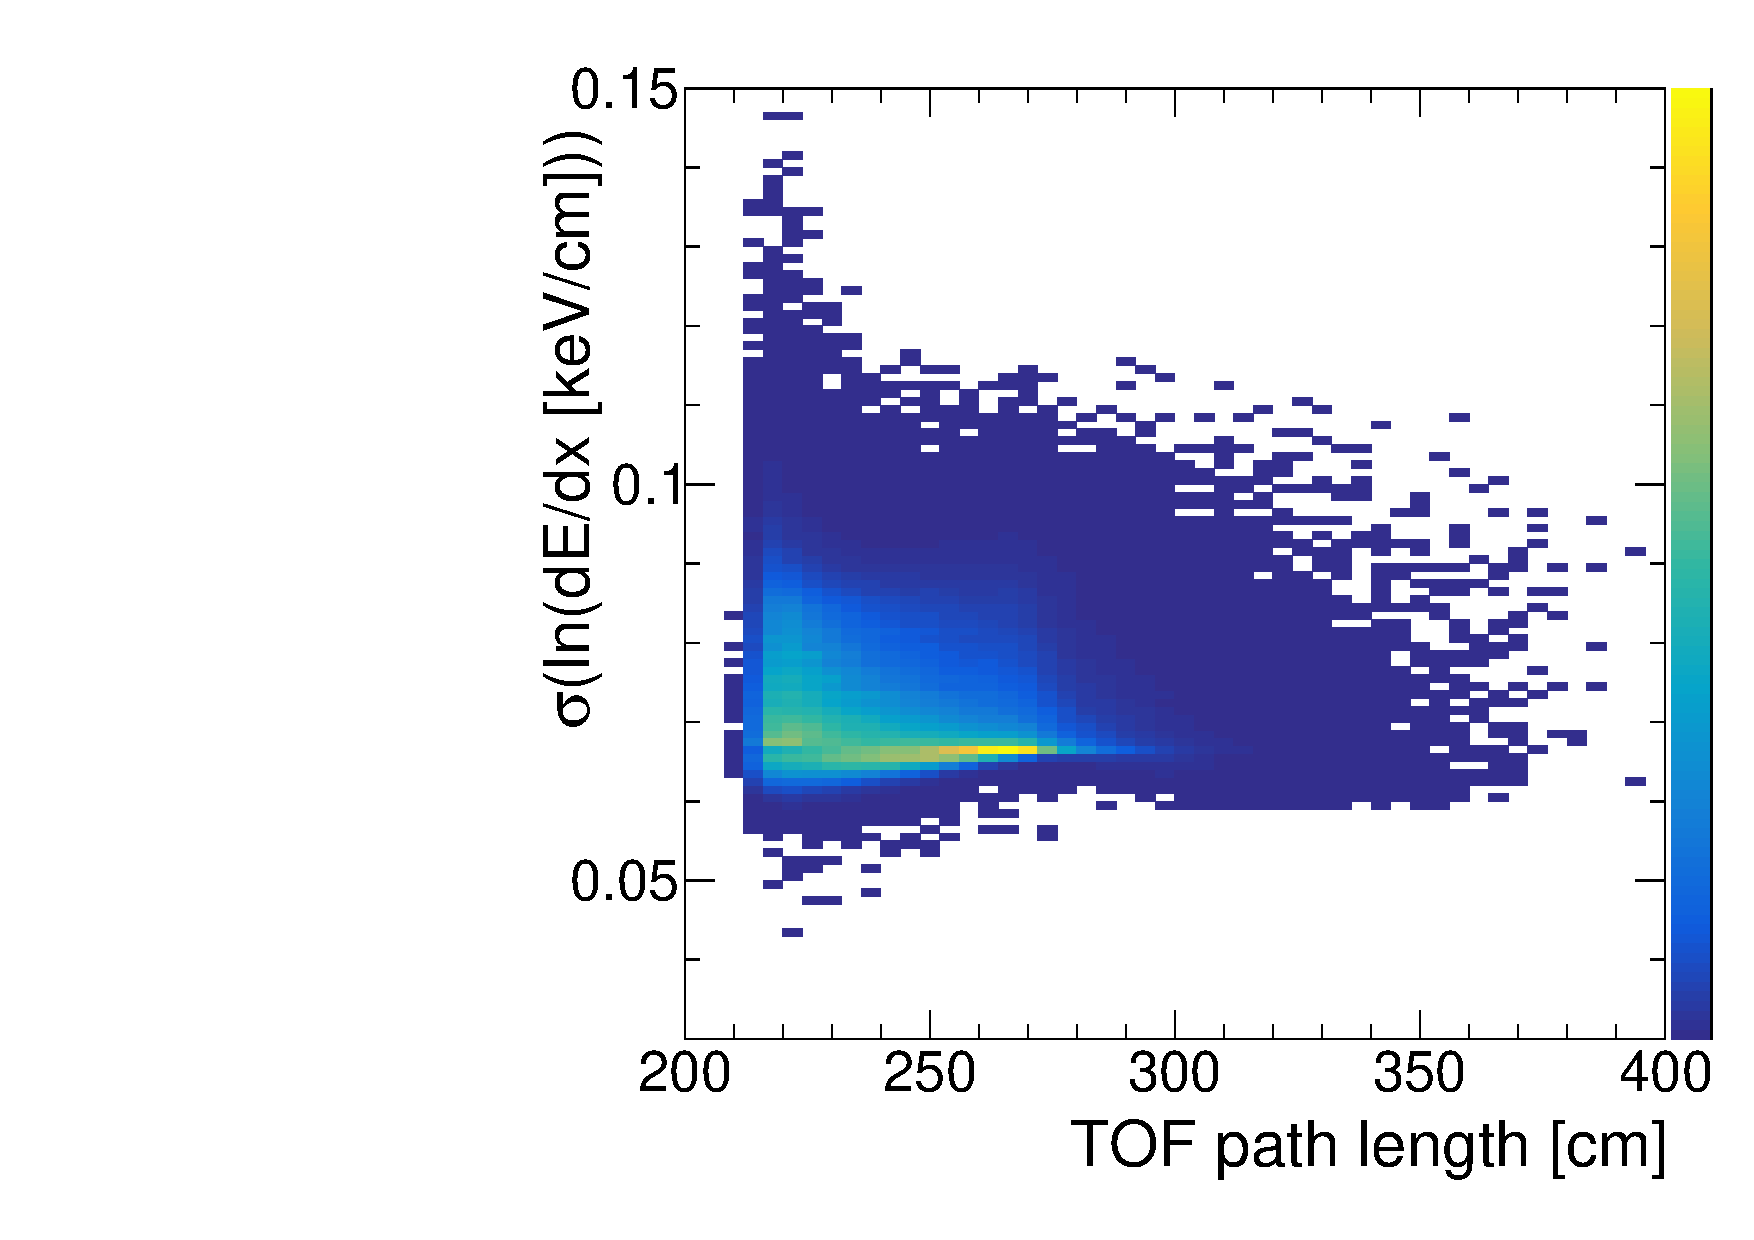
\includegraphics[width=\linewidth]{graphics/corrections/DEdxErrorVsTofPathLength.pdf}}}
  \end{subfigure}
}
\quad
\parbox{0.4725\textwidth}{
  \centering
  \begin{subfigure}[b]{\linewidth}{
                \subcaptionbox{\label{fig:Log2dEdxVsTofPathLength}}{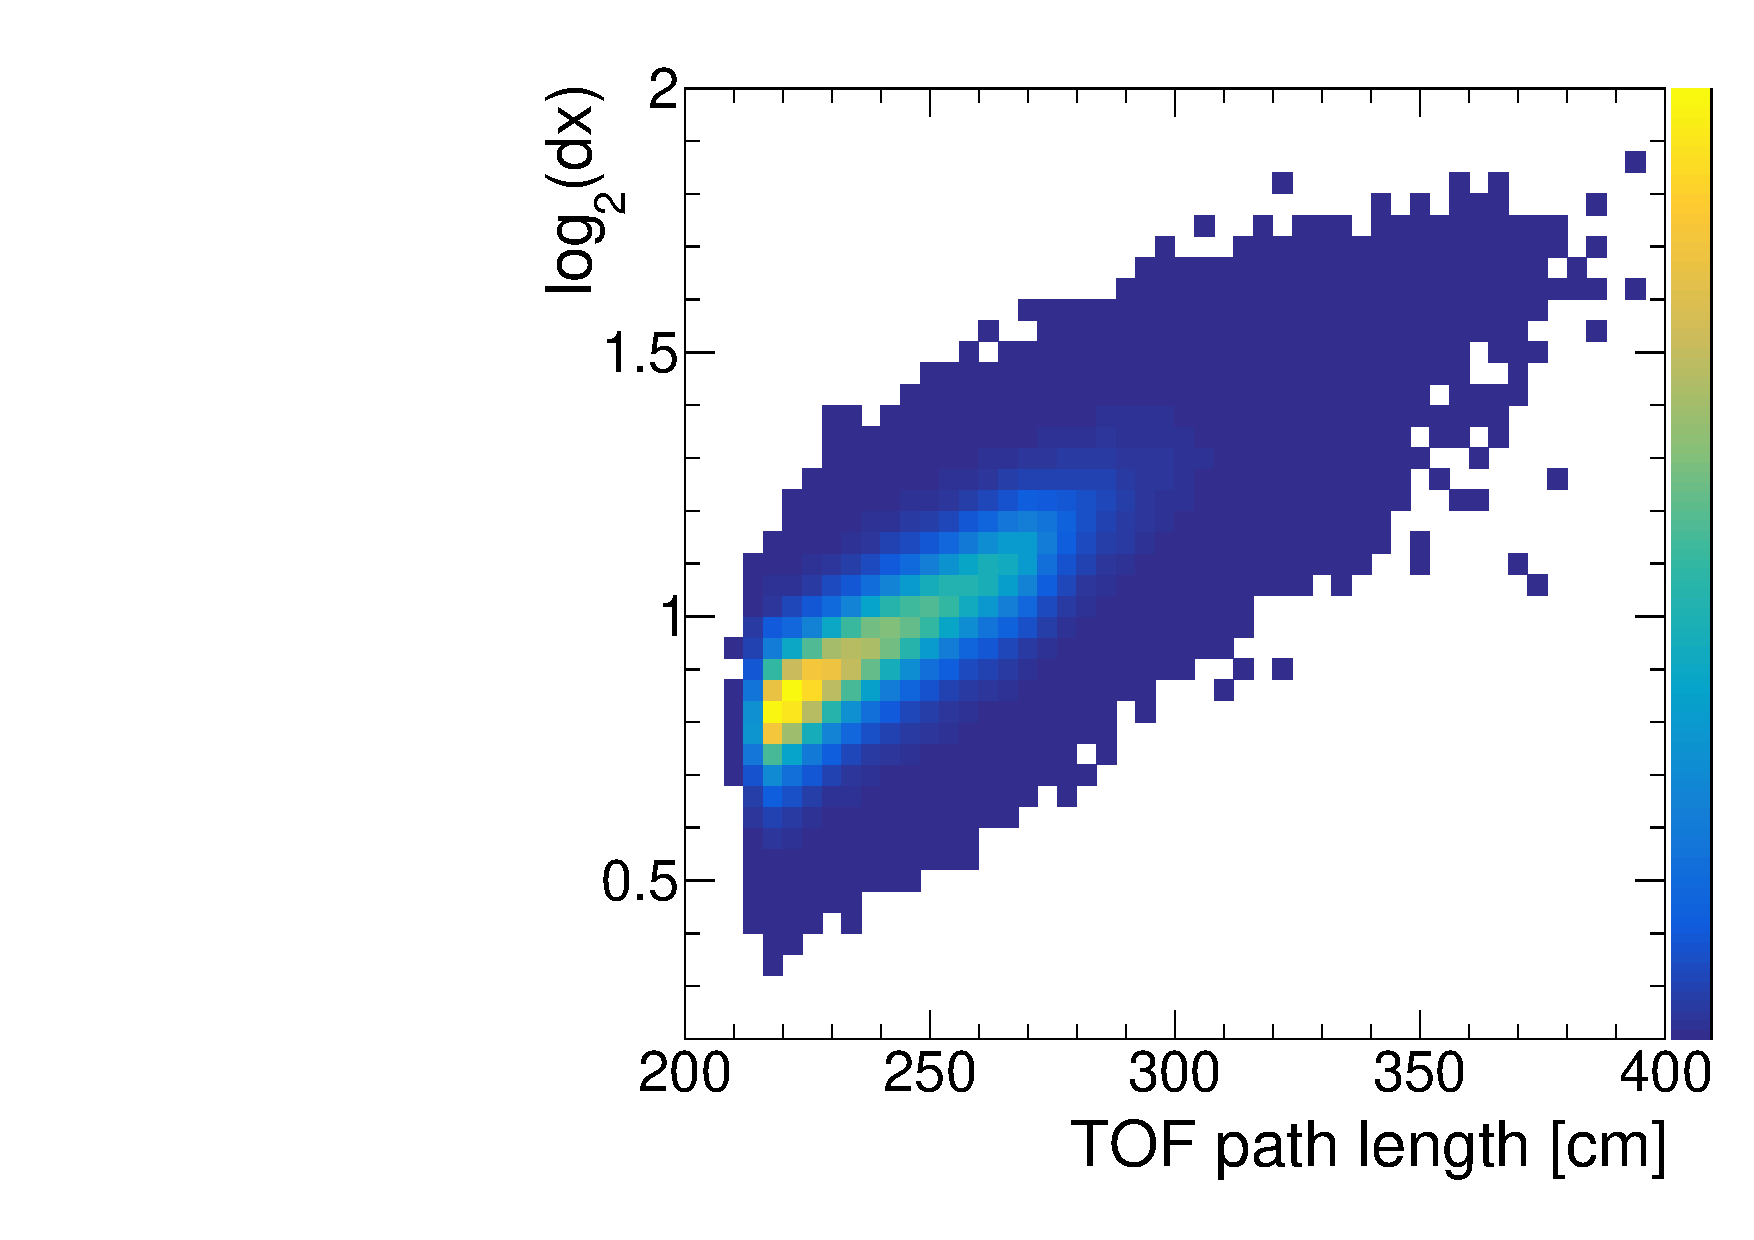
\includegraphics[width=\linewidth]{graphics/corrections/Log2dxVsTofPathLength.pdf}}}
  \end{subfigure}
}% 
\caption[$dE/dx$ error vs. TOF path length and $\log_{2}(dx)$ vs. TOF path length for exclusive event candidates.]{Correlation between uncertainty of the natural logarithm of $dE/dx / (1~\text{keV/cm})$ and track TOF path length (\ref{fig:dEdxErrorVsTofPathLength}) and correlation between base 2 logarithm of $dx$ and track TOF path length (\ref{fig:Log2dEdxVsTofPathLength}). The distributions were obtained for the exclusive event candidates after full selection, with all three types of particle pairs combined.} \label{fig:correlationsTofPathLength}
\end{figure} 


For the purpose of determination of pair identification efficiency in CEP analysis descibed in this note, parameters of vertex distribution were set to match the data: $\langle z_{\text{vtx}}\rangle=0$ and $\sigma(z_{\text{vtx}})=50$~cm, as well as $z_{\text{vtx}}$ was required to lie within the analysis limits (cut~\ref{enum:CutZVx}). Distribution of particle $\eta$ was set to flat and limited to analyzed range $|\eta|<0.7$, while particle $\phi$ was defined as uniformly distributed in full azimuth ($2\pi$~rad), both fairly agreeing with expectations from physics models and observations in data.

\section{Background modelling}\label{sec:mcBkgdContrib}

The following MC samples were used in this study:
\begin{itemize}
 \item CD (background) - Central Diffraction events from Pythia~8.1 generator with MBR model of \Pom omeron flux, filtered at generation to ensure lack of signal in BBC-large, passed through Geant3 simulation of the STAR detector (STARsim) and Geant4 simulation of the RP Phase II* detectors, partially embedded into zero-bias data (only the simulated RP response embedded),%\vspace*{-5pt}
 \item MB+elastic, (background) - Minimum Bias events from Pythia~8.1 generator with MBR model of \Pom omeron flux, filtered at generation to ensure lack of signal in BBC-large, passed through Geant3 simulation of the STAR detector (STARsim) and Geant4 simulation of the RP Phase II* detectors, partially embedded into elastic trigger (RP\_ET) data (only the simulated RP response embedded).%\vspace*{-5pt}
\end{itemize}

Listed background samples were not fully embedded since an enormous CPU time would be required to obtain satisfactory statistics. It was also found unnesessary to embed TPC tracks into zero-bias data to obtain reliable agreement between distributions of desired quantities presented below.

MC samples from Pythia generator were additionally filtered before passing through Geant to increase generation efficiency, as well as overcome difficulty arising from missing simulation of the BBC-large in STARsim. For each event, all charged particles were analytically propagated through the magnetic field of TPC with the helical paths resulting from their hadron-level momenta. If any of these particles crossed the volume of BBC-large detector, event was dropped from generation.


%% %% %% %% %% %% %% %% %% %% %% %% %% %% %% %% %% %% %% %% %% %% %% %% %% %% %% %% %% %% %% %% %% %% %% %% 
\section{Model predictions}\label{sec:mcModelPred}

\subsection{GenEx}
The GenEx~\cite{GenEx} and DiMe~\cite{DurhamModel} event generators are based on a simple phenomenological models~\cite{LSmodel, LSModelKK, harland_lang_1} of continuum production mechanism of $\pi^+\pi^-$ or $K^+K^-$ pairs. In the model implemented in GenEx the absorption corrections are not taken into account explicitly. A damping factor was estimated to be of the order of 2-5 ($\pi^+\pi^-$) and 2 ($K^+K^-$)~\cite{LSAbsorption}. To account for absorption the cross sections obtained from GenEx are scaled by 0.35 and 0.6 for $\pi^+\pi^-$ and $K^+K^-$, respectively, to fit DiMe predictions which include absorption effects. Predictions are also sensitive to the choice of meson form factor. GenEx predictions are shown using exponential form factor with $\Lambda_{of\!f}^{2}=1.0~\textrm{GeV}^{2}$. Changes of $\Lambda_{of\!f}^{2}$ by 50\% lead to cross section changes up to a factor of 2.

\subsection{DiMe}
In the DiMe event generator four models for absorption are available. The prediction from "model 2" giving the best consistency with data is used in the following. DiMe predictions are also sensitive to the choice of meson form factor. Three different parameterizations of meson form factor are implemented. We chose exponential form with the same slope as used for GenEx predictions. Therefore the differences between GenEx and DiMe are almost entirely due to the absorption.

\subsection{Pythia8 MBR}
The MBR model~\cite{mbr_pythia8} implemented in PYTHIA8~\cite{pythia8} was founded to describe inclusive 
central diffarction (CD, $p+p\rightarrow P+X+p$ cross section 
at CDF while exclusive $h^+h^-$ state occurs from fragmentation and hadronization of the central state based on the Lund string model. MBR model implemented in PYTHIA8.165 allows generation of the central state starting from the mass threshold of $2 m_h$. In later versions region below 1~GeV mass was excluded. Therefore PYTHIA8 expectations for very low masses are in question but are shown for completeness.
